\section{Results}
\label{sec:results}

This section will outline the results of our efforts in this project including the metrics of the model itself and an example of it's working state. \\

We
\begin{figure}[h]
    \centering
    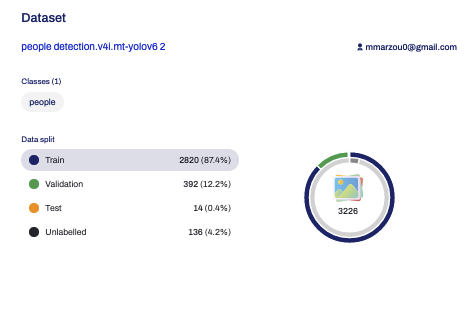
\includegraphics[width=0.5\textwidth]{images/train.png}
    \caption{training data}
    \label{fig:data}
\end{figure}

\begin{figure}[h]
    \centering
    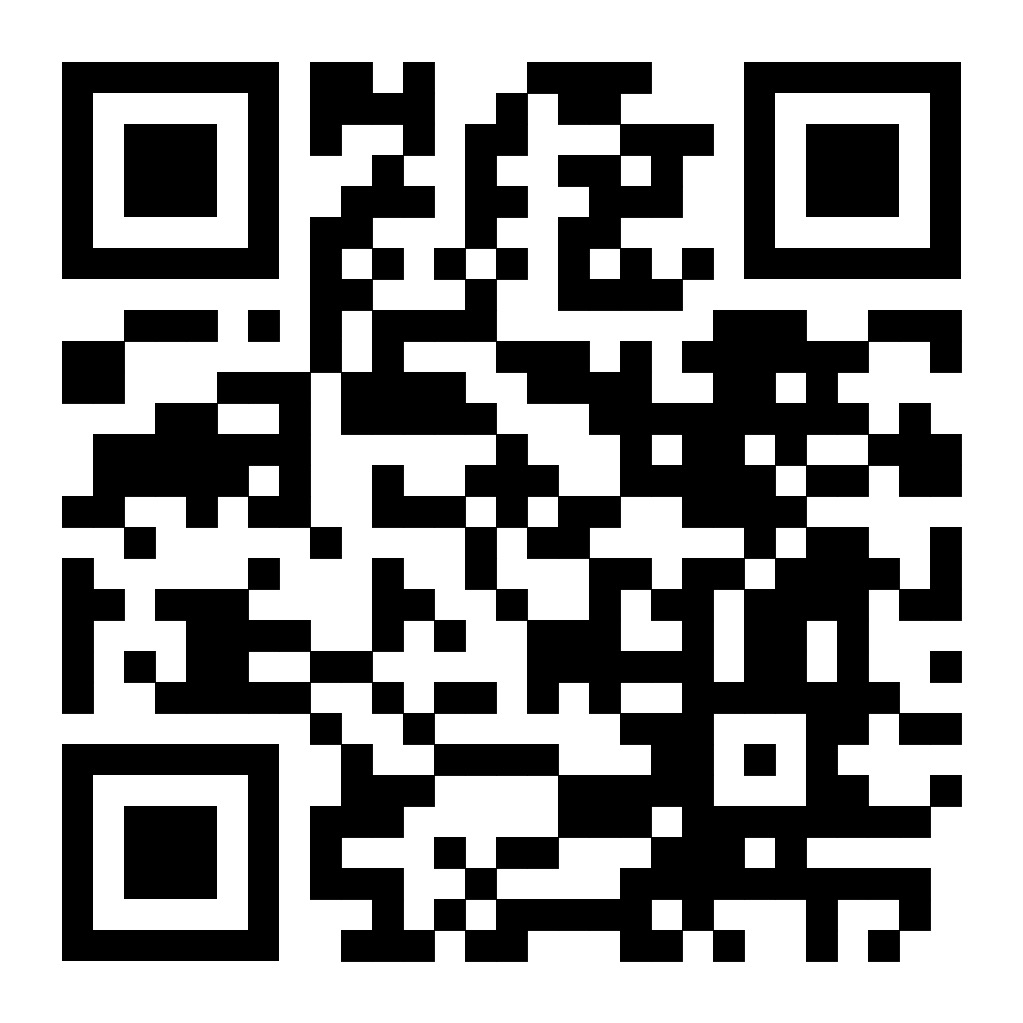
\includegraphics[width=0.5\textwidth]{images/QR.png}
    \caption{QR code for Demo}
    \label{fig:data}
\end{figure}

Prior to loading any images, we implemented a pre-processing step to stitch images to ensure that all the images are the same size. The images were stitched together using the OpenCV. \\
\begin{figure}[h]
    \centering
    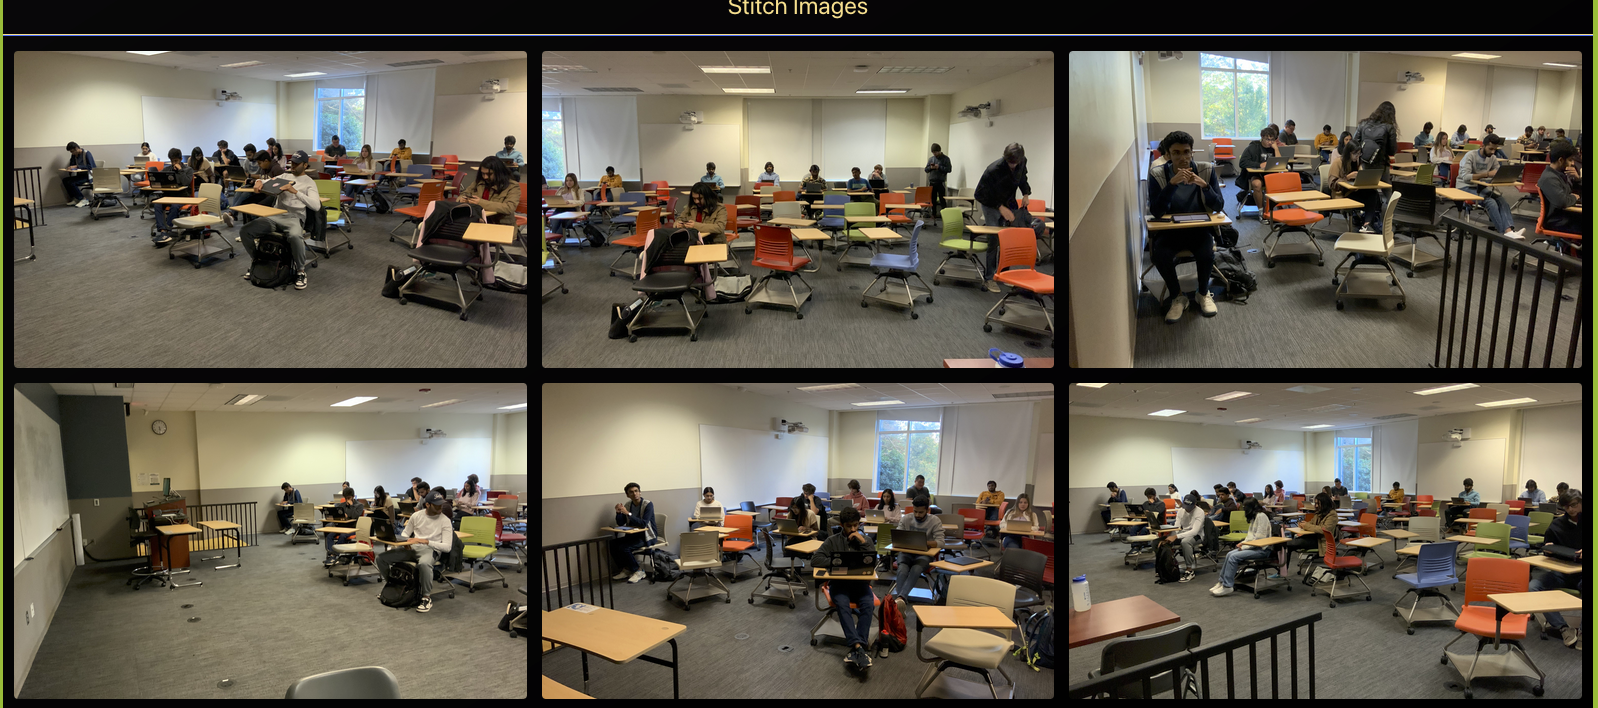
\includegraphics[width=0.5\textwidth]{images/Pre.png}
    \caption{Pre-Processed Image}
    \label{fig:before}
\end{figure}

After the image is pre-processed, it is fed into the model. The image below shows the image before it is fed into the model. \\
\begin{figure}[h]
    \centering
    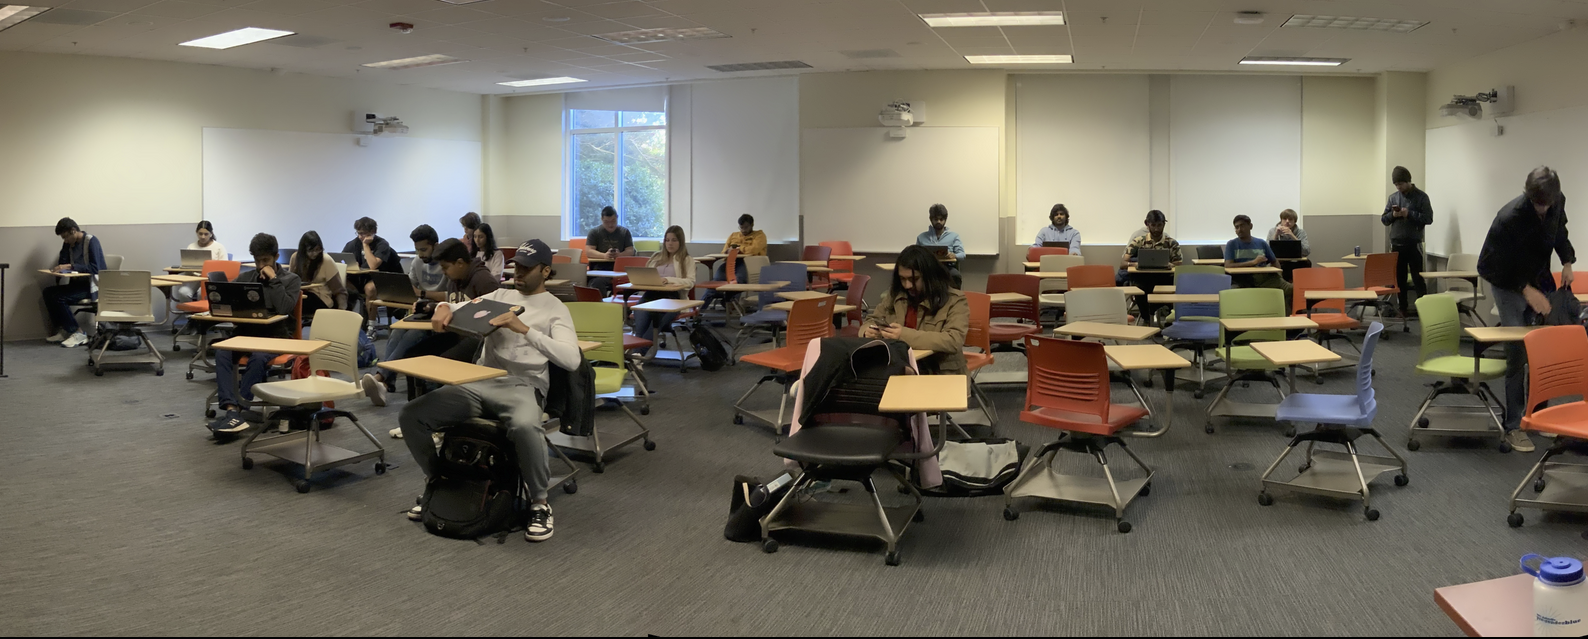
\includegraphics[width=0.5\textwidth]{images/Before.png}
    \caption{Before}
    \label{fig:before}
\end{figure}

The image below shows the results of the model. The model was trained for 100 epochs and the loss was 0.0001. The model that was used was pre-trained on yolov6-n variant of the YOLO family. \\

\begin{figure}[h]
    \centering
    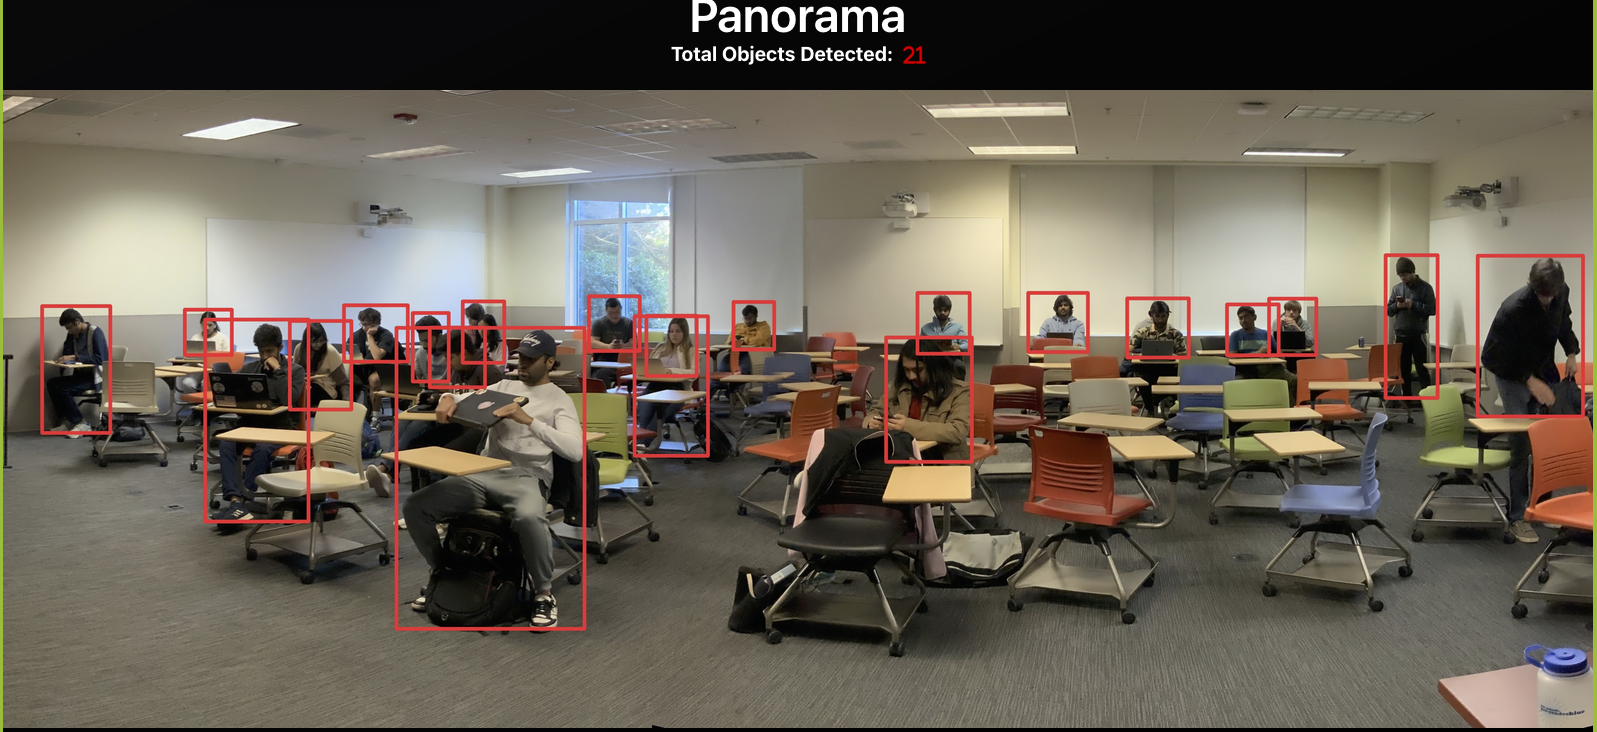
\includegraphics[width=0.5\textwidth]{images/After.png}
    \caption{After}
    \label{fig:after}
\end{figure}

%-------------------------------------------------------------------------
